% Created:  Wed 09 Jul 2014 03:00 PM
% @author Josh Wainwright
% File name : clusters.tex

\chapter{Existing Cluster Analysis Algorithms}
\label{prt:existing_cluster_analysis_algorithms}

Cluster analysis is the grouping of a set of objects or items in a spatially or
informationally logical way such that the items that are placed in the same
group are more similar to each other than they are to the objects in the other
groups in the set. These groups shall be called \emph{clusters}. When dealing
with images, the clustering that is of interest is often based on spatial
location, i.e., clusters should be composed of objects that are close together
in the image and clusters should be separated by regions of emptiness or
background level noise.

A number of clustering algorithms already exist. Many of these are designed for
very specific purposes and so are not well suited for this application. Several
of these are described below.

\section{Rolling Ball Analysis}
\label{sub:rolling_ball_analysis}

The accessible surface area (ASA) algorithm, also known as the ``Rolling Ball
Method'', is a technique used in image processing for describing the outer
limit of a cluster of points. It is derived from biological molecules analysis
where it describes the surface area of a molecule that is accessible to a
liquid solvent.

The rolling ball method can be used to analyse a cluster of points by imagining
a solid ball or circle that sits against one of the outer-most points. From
here it is ``rolled'' around the cluster such that it is always touching at
least one point. Once the ball has reached the point it started from, the line
that the ball traced is reduced in size by the radius of the ball. This line
then represents the outer limit of the cluster.

The size of the ball must be chosen depending on the average separation of the
points within the cluster such that points classed as noise are not included
but all interesting points are.

\begin{figure}[tbh]
	\centering
	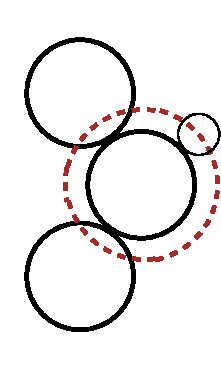
\includegraphics[width=4.0cm]{rolling-ball.pdf}

	\caption[Rolling ball method for cluster analysis.]{The rolling ball method
		for cluster detection provides a way of identifying clusters, as
		inspired by molecular biology. A very simple implementation can be fast
		but is not particularly successful at finding clusters unless the data
		points are very dense and there is no noise.}\label{fig:rolling-ball}
\end{figure}

A simple approximation of this technique can be achieved by using the same
dilating and eroding processes that are described later in
Section~\ref{sec:simple_grid_method}.

\section{Shared Nearest Neighbours}
\label{sub:shared_nearest_neighbours}

Shared nearest neighbour (SNN) clustering algorithms have been used to overcome
some of the problems encountered with more traditional clustering methods when
working in higher dimensions. In these cases, simple Euclidean geometry becomes
unable to cope with the computation and so is replaced with other coordinate
systems. For simple clustering in two dimensions, however, Euclidean geometry
is sufficient and is far easier and more efficient to implement.

SNN based clustering algorithms analyse each of the points in a set, selecting
those points that lie close to the current one based on certain thresholds. As
the algorithm progresses, these thresholds are altered and the points
considered so far are re-examined to maximise the `similarity' of the points
in any one cluster.

Implementations of SNN based algorithms, such as~\cite{jarvis1973clustering}
and~\cite{ertoz2002new} use similarity matrices, where the set of points is
reduced to a graph with data points at nodes and edges between them
representing the similarities between the points. This matrix is then
simplified to leave a sparse graph, keeping only the edges with the highest
similarity. From this matrix, points can be identified as noise and rejected,
and the networks that show close similarities are designated as clusters.

This method is very good at being adaptable to complex situations such as
arbitrary dimension or clusters with complicated shapes. However, the
complexity in implementation and computation makes it unsuitable for small
scale clustering such as the application discussed for this project. It also
suffers from performance issues when the number of points to analyse becomes
large as it has approximately $O(n^2)$ time complexity.

\section{Gravity Based Clustering}
\label{sub:gravity_based_clustering}

A number of clustering algorithms~\cite{zhong2010novel} have been developed
that treat data points as physical objects under the influence of gravitational
effects. These algorithms effectively model the points with these properties,
allow them to move with some defined restrictions, and then examine the
products that are produced.

The GRAVIclust algorithm~\cite{indulska2002gravity} works in two phases, first
identifying $n$ locations of interest based on the distances to neighbouring
points, similar to the SNN algorithms above, and secondly applying an
optimisation phase where each of these locations is further examined with the
gravity effects of other points applied.

Unfortunately, these algorithms require certain information about the data set
before clustering can be performed. First, a matrix of the distances between
every pair of points must be calculated. This makes working with large data
sets prohibitive. Secondly, the number of clusters to identify is required.
This means that an algorithm to search for arbitrary numbers of clusters is not
possible.
